\section{Image Reconstruction for Interferometers}\label{intro}
The angular resolution of a radio antenna is proportional to the wavelength divided by the dish diameter. To achieve high angular resolution the diameter should be as large as possible. But real world limitations like steering accuracy and price limit the diameter. Currently the largest single dish antenna has a diameter of about 500 meters\cite{chinaFAST}. 
  
Interferometers however, achieve high angular resolutions without the need for huge dish diameters. Several smaller antennas are spaced apart from each other. Together, they act as a single antenna. Interferometers have seen wide use in for radio wavelengths with instruments like VLA and LOFAR.

Interferometers do not observe the sky directly. The observed image has to be reconstructed from the measurements. The reconstruction is an ill-posed inverse problem. In Radio Astronomy, the CLEAN class of algorithms\cite{hogbom1974aperture}\cite{schwab1984relaxing}\cite{rich2008multi}\cite{rau2011multi} are used to reconstruct the image and is the de-factor standard. 

Fixed assumption about the image

New Interferometers on the horizon with SKA. To improve reconstruction, we would like to model our prior knowledge about the. New observations new effects. CLEAN has a rigid assumption about what the reconstructed image should look like. It cannot be adapted as our knowledge of the universe changes.

The Theory of Compressed Sensing\cite{candes2006robust}\cite{donoho2006compressed} has seen success in solving ill-posed inverse problems. 

It is flexible in its application and can be used in de-noising\cite{many}, in-painting\cite{many} and super-resolution\cite{many}.

Using prior knowledge about the reconstructed image. 
Push to a plausible image reconstruction

%Applying Compressed Sensing to wide Field of View imaging is an active field of research. In the last decade numerous approaches have been developed showing the potential of Compressed Sensing: Accurately modelling the effects of wide Field of View imaging, while reducing the tunable parameters and possibly super-resolved images\cite{garsden2015lofar}. Current research focuses on how the effects of wide Field of View can be accurately modelled while still being computationally efficient.

In this project, a proof of concept Compressed Sensing reconstruction algorithm was developed and implemented in the Common Astronomy Software Application(CASA). 


\subsection{Deconvolution: Ill-posed Inverse Problem}
Interferometers do not observe the image directly. Instead, they measure approximately three dimensional Fourier components. An accurate measurement equation and are important for wide field of view imaging. In this project small field of view reconstruction was considered. For small field of View, the measurement equation can be approximated by the two dimensional Fourier Components(Visibility). Each antenna pair measures a complex Visibility. Therefore the observed image can be calculated from the (small field of view) observations by using the two dimensional Fourier Transform.

If the interferometer could sample all Visibilities, then the Fourier Transform would produce the observed image. However, since there are a limited number of antenna pairs, we  measure the same limited number of Visibilities. The measurement is under-sampled and the image of the Fourier Transform is "dirty". The undersampling convolves the observed image with a point spread function(PSF). The task is to deconvolve the image and remove the effects of undersampling \eqref{intro:eq:deconvolve}.

\begin{equation}\label{intro:eq:deconvolve}
x \star  PSF + N = I_{dirty} 
\end{equation}

the PSF models the instrumental effects of undersampling, antenna beam patterns.
The point spread function models the instrument effects. The task is now to deconvolve the image in a noisy environment.  .

Equation \eqref{intro:eq:deconvolve} is an ill posed problem::
\begin{itemize}
	\item It is unknown if a solution exists
	\item There may be many solutions
	\item a small change in the measurement may lead to very different solutions 
\end{itemize}

incoherence


CASA produces a the $I_{dirty}$ image and the PSF.


%Each antenna pair measures a complex Visibility of the sky brightness. The distance between the antennas, the baseline, dictates the sample point in the Fourier Space (called UV-Space). Longer baselines sample higher frequency components, while shorter baselines sample lower frequency components. 

%For small Field of View imaging, the measured Visibilities equal two dimensional Fourier components. The observed image can be calculated by the two dimensional Inverse Fourier Transform. However the interferometer cannot sample the whole UV-Space. The image calculated by the Inverse Fourier Transform is 'dirty', it contains artefacts introduced by undersampling. 

\begin{figure}[h!]
	\centering
	\begin{subfigure}[b]{0.28\linewidth}
		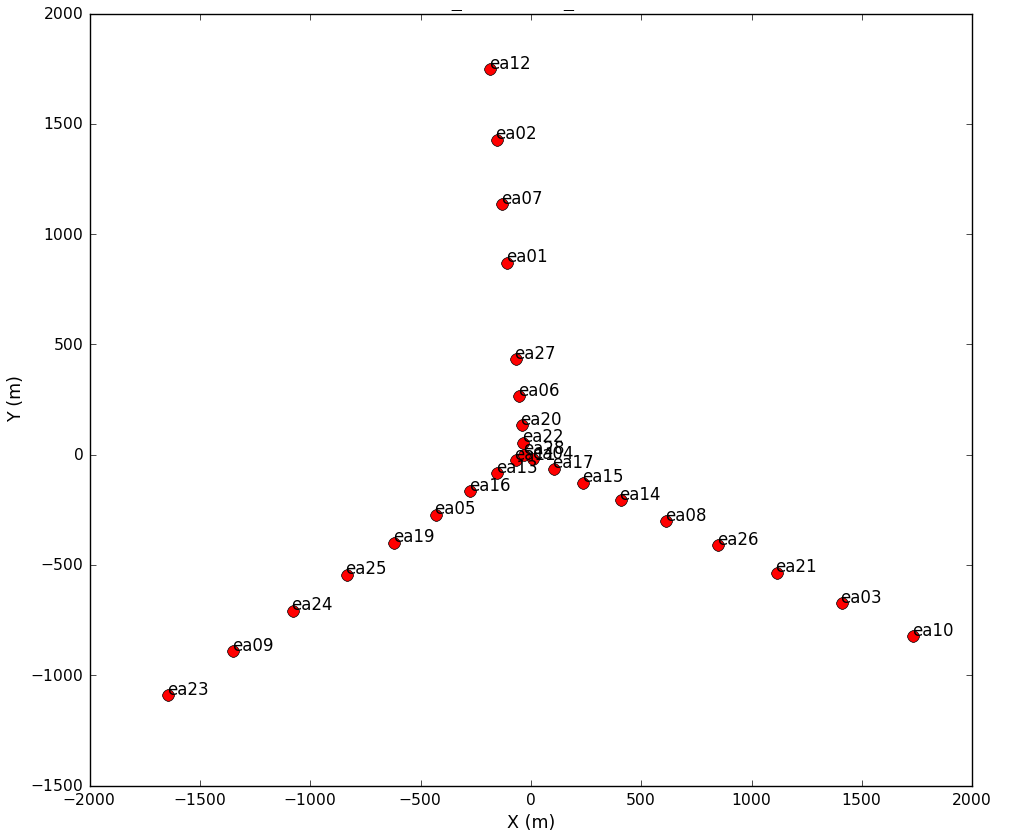
\includegraphics[width=\linewidth, trim={18px 19px 18px 18px}, clip]{./chapters/01.intro/img/antennas.png}
		\caption{Antenna Configuration}
	\end{subfigure}
	\begin{subfigure}[b]{0.28\linewidth}
		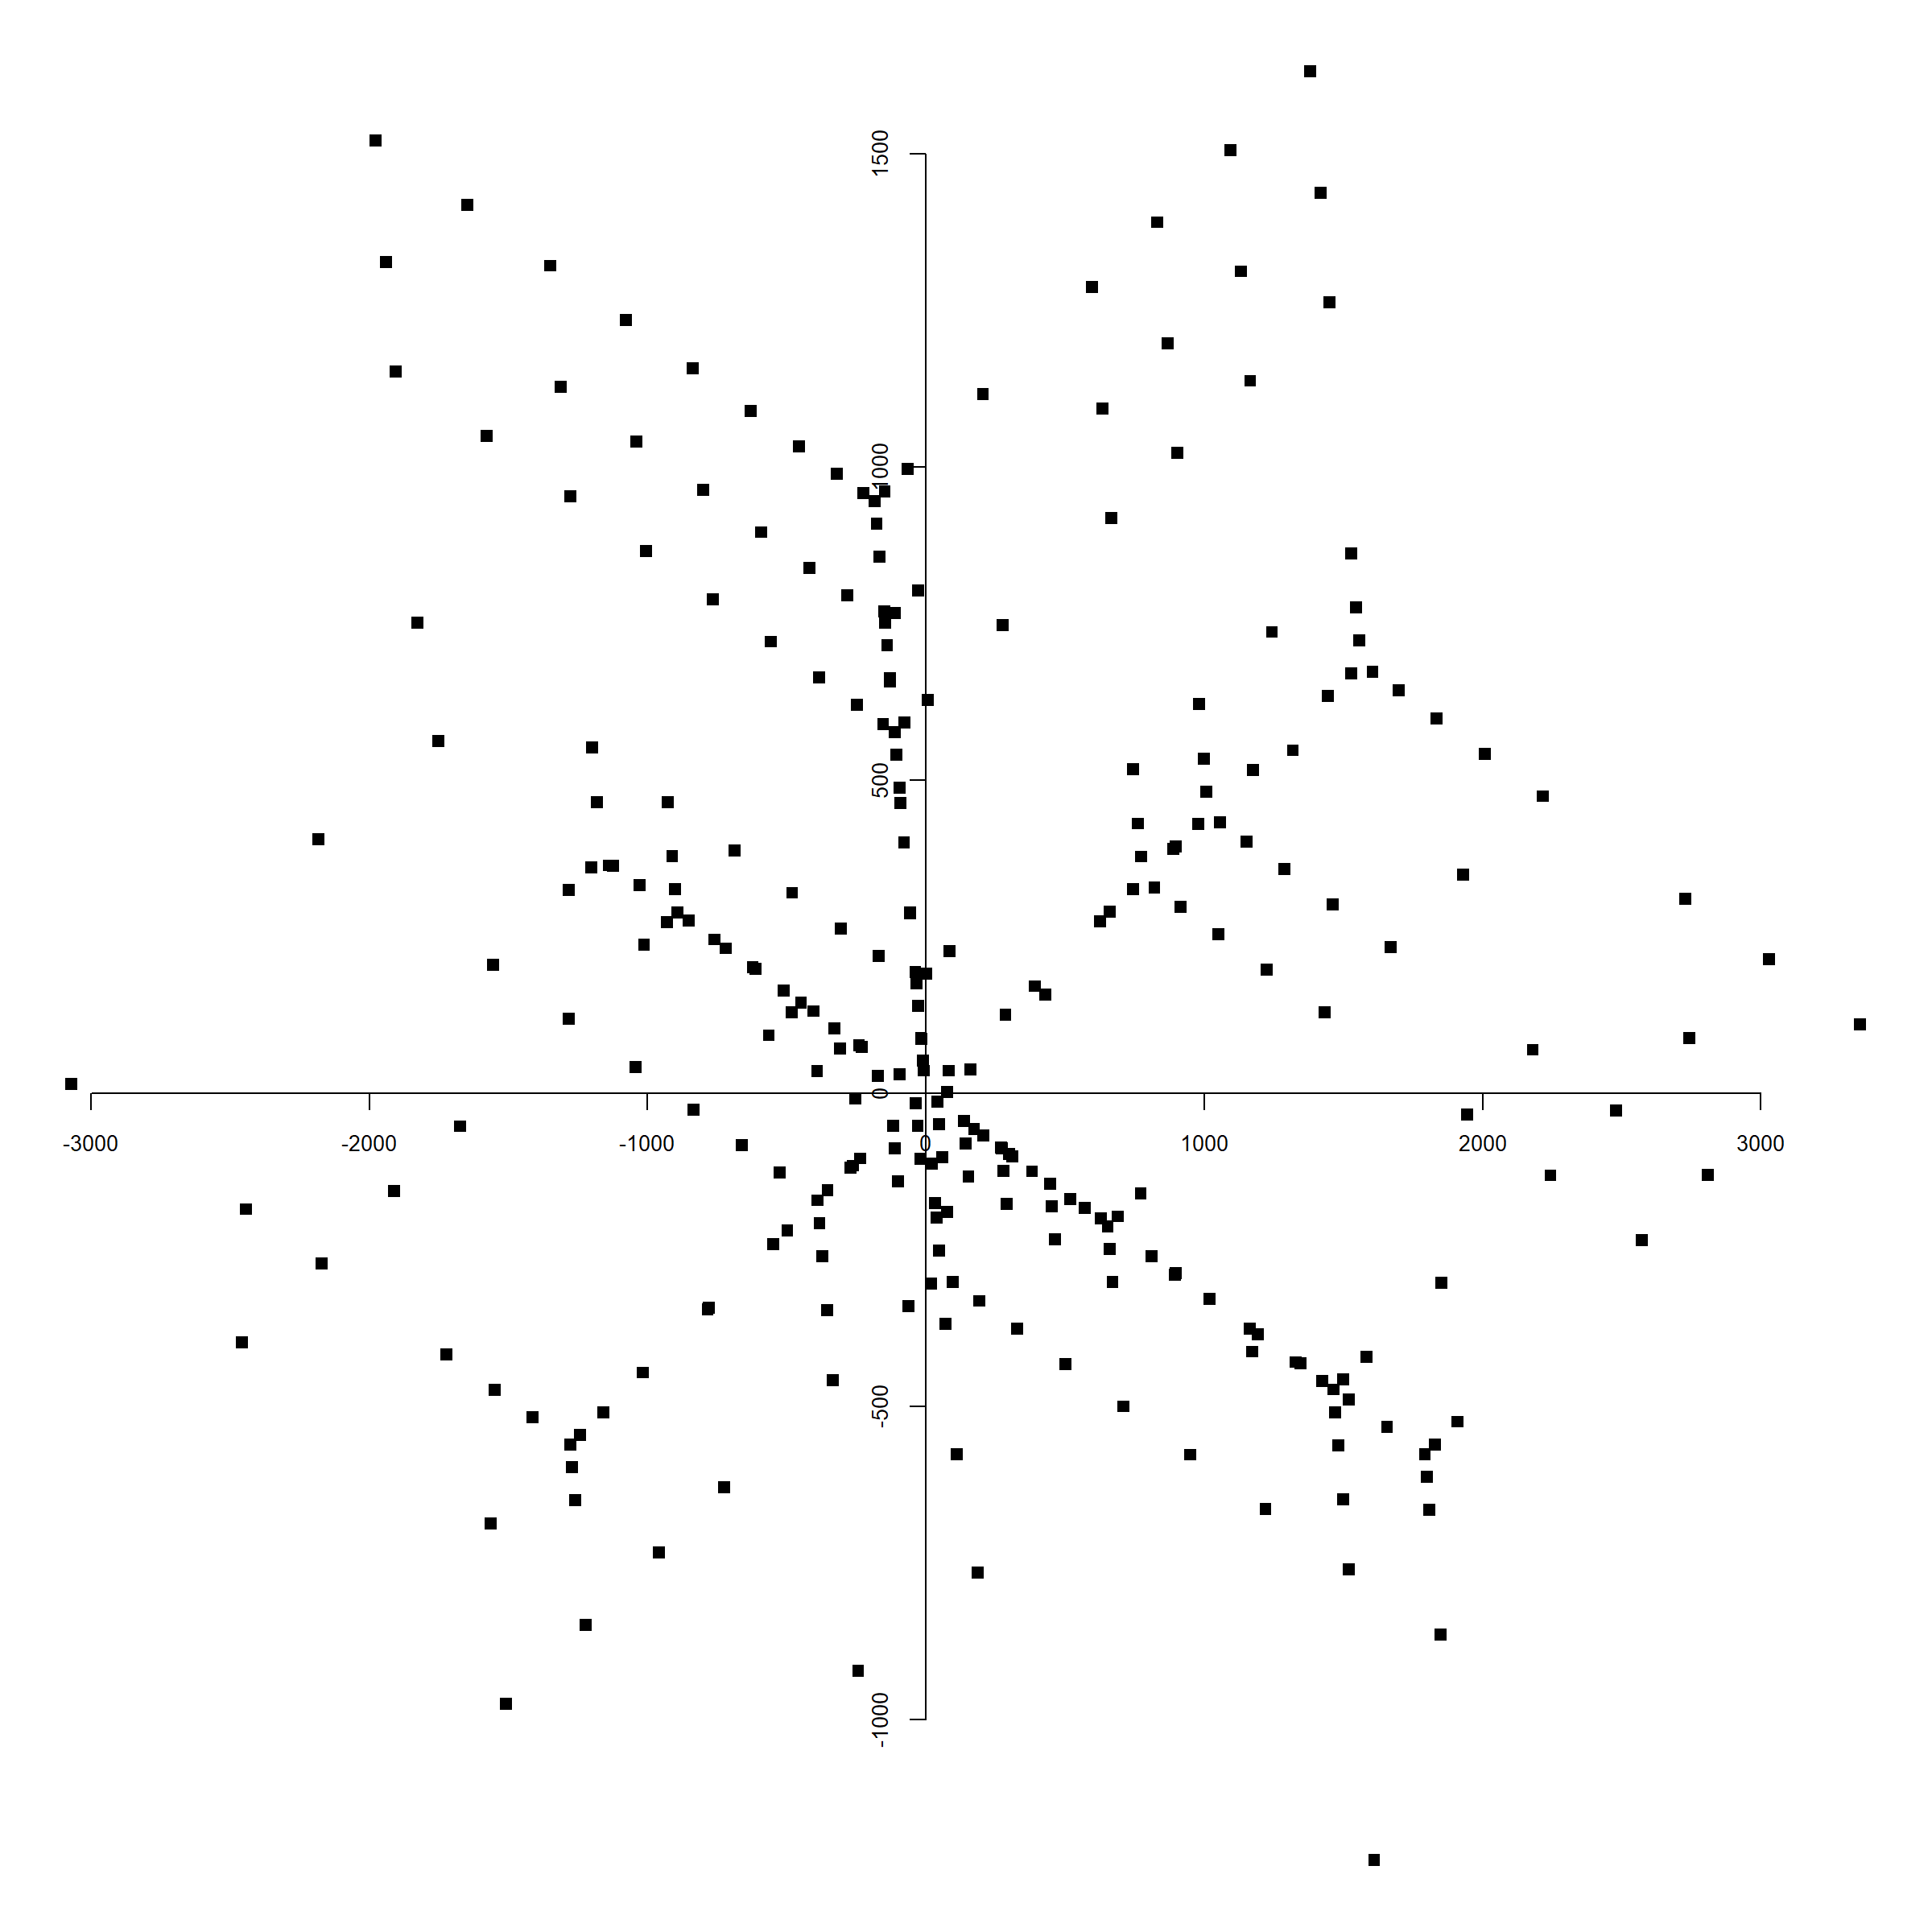
\includegraphics[width=\linewidth, trim={18px 19px 18px 18px}, clip]{./chapters/01.intro/img/uv.png}
		\caption{UV-Space}
	\end{subfigure}

	\begin{subfigure}[b]{0.28\linewidth}
		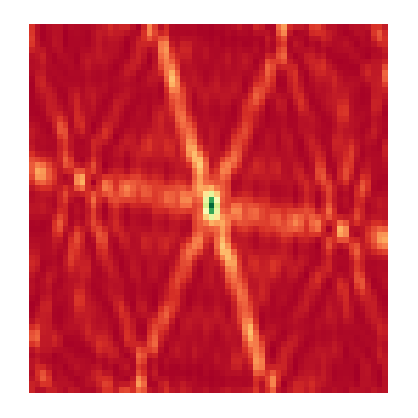
\includegraphics[width=\linewidth, trim={18px 19px 18px 18px}, clip]{./chapters/01.intro/img/psf.png}
		\caption{PSF}
	\end{subfigure}
	\begin{subfigure}[b]{0.28\linewidth}
		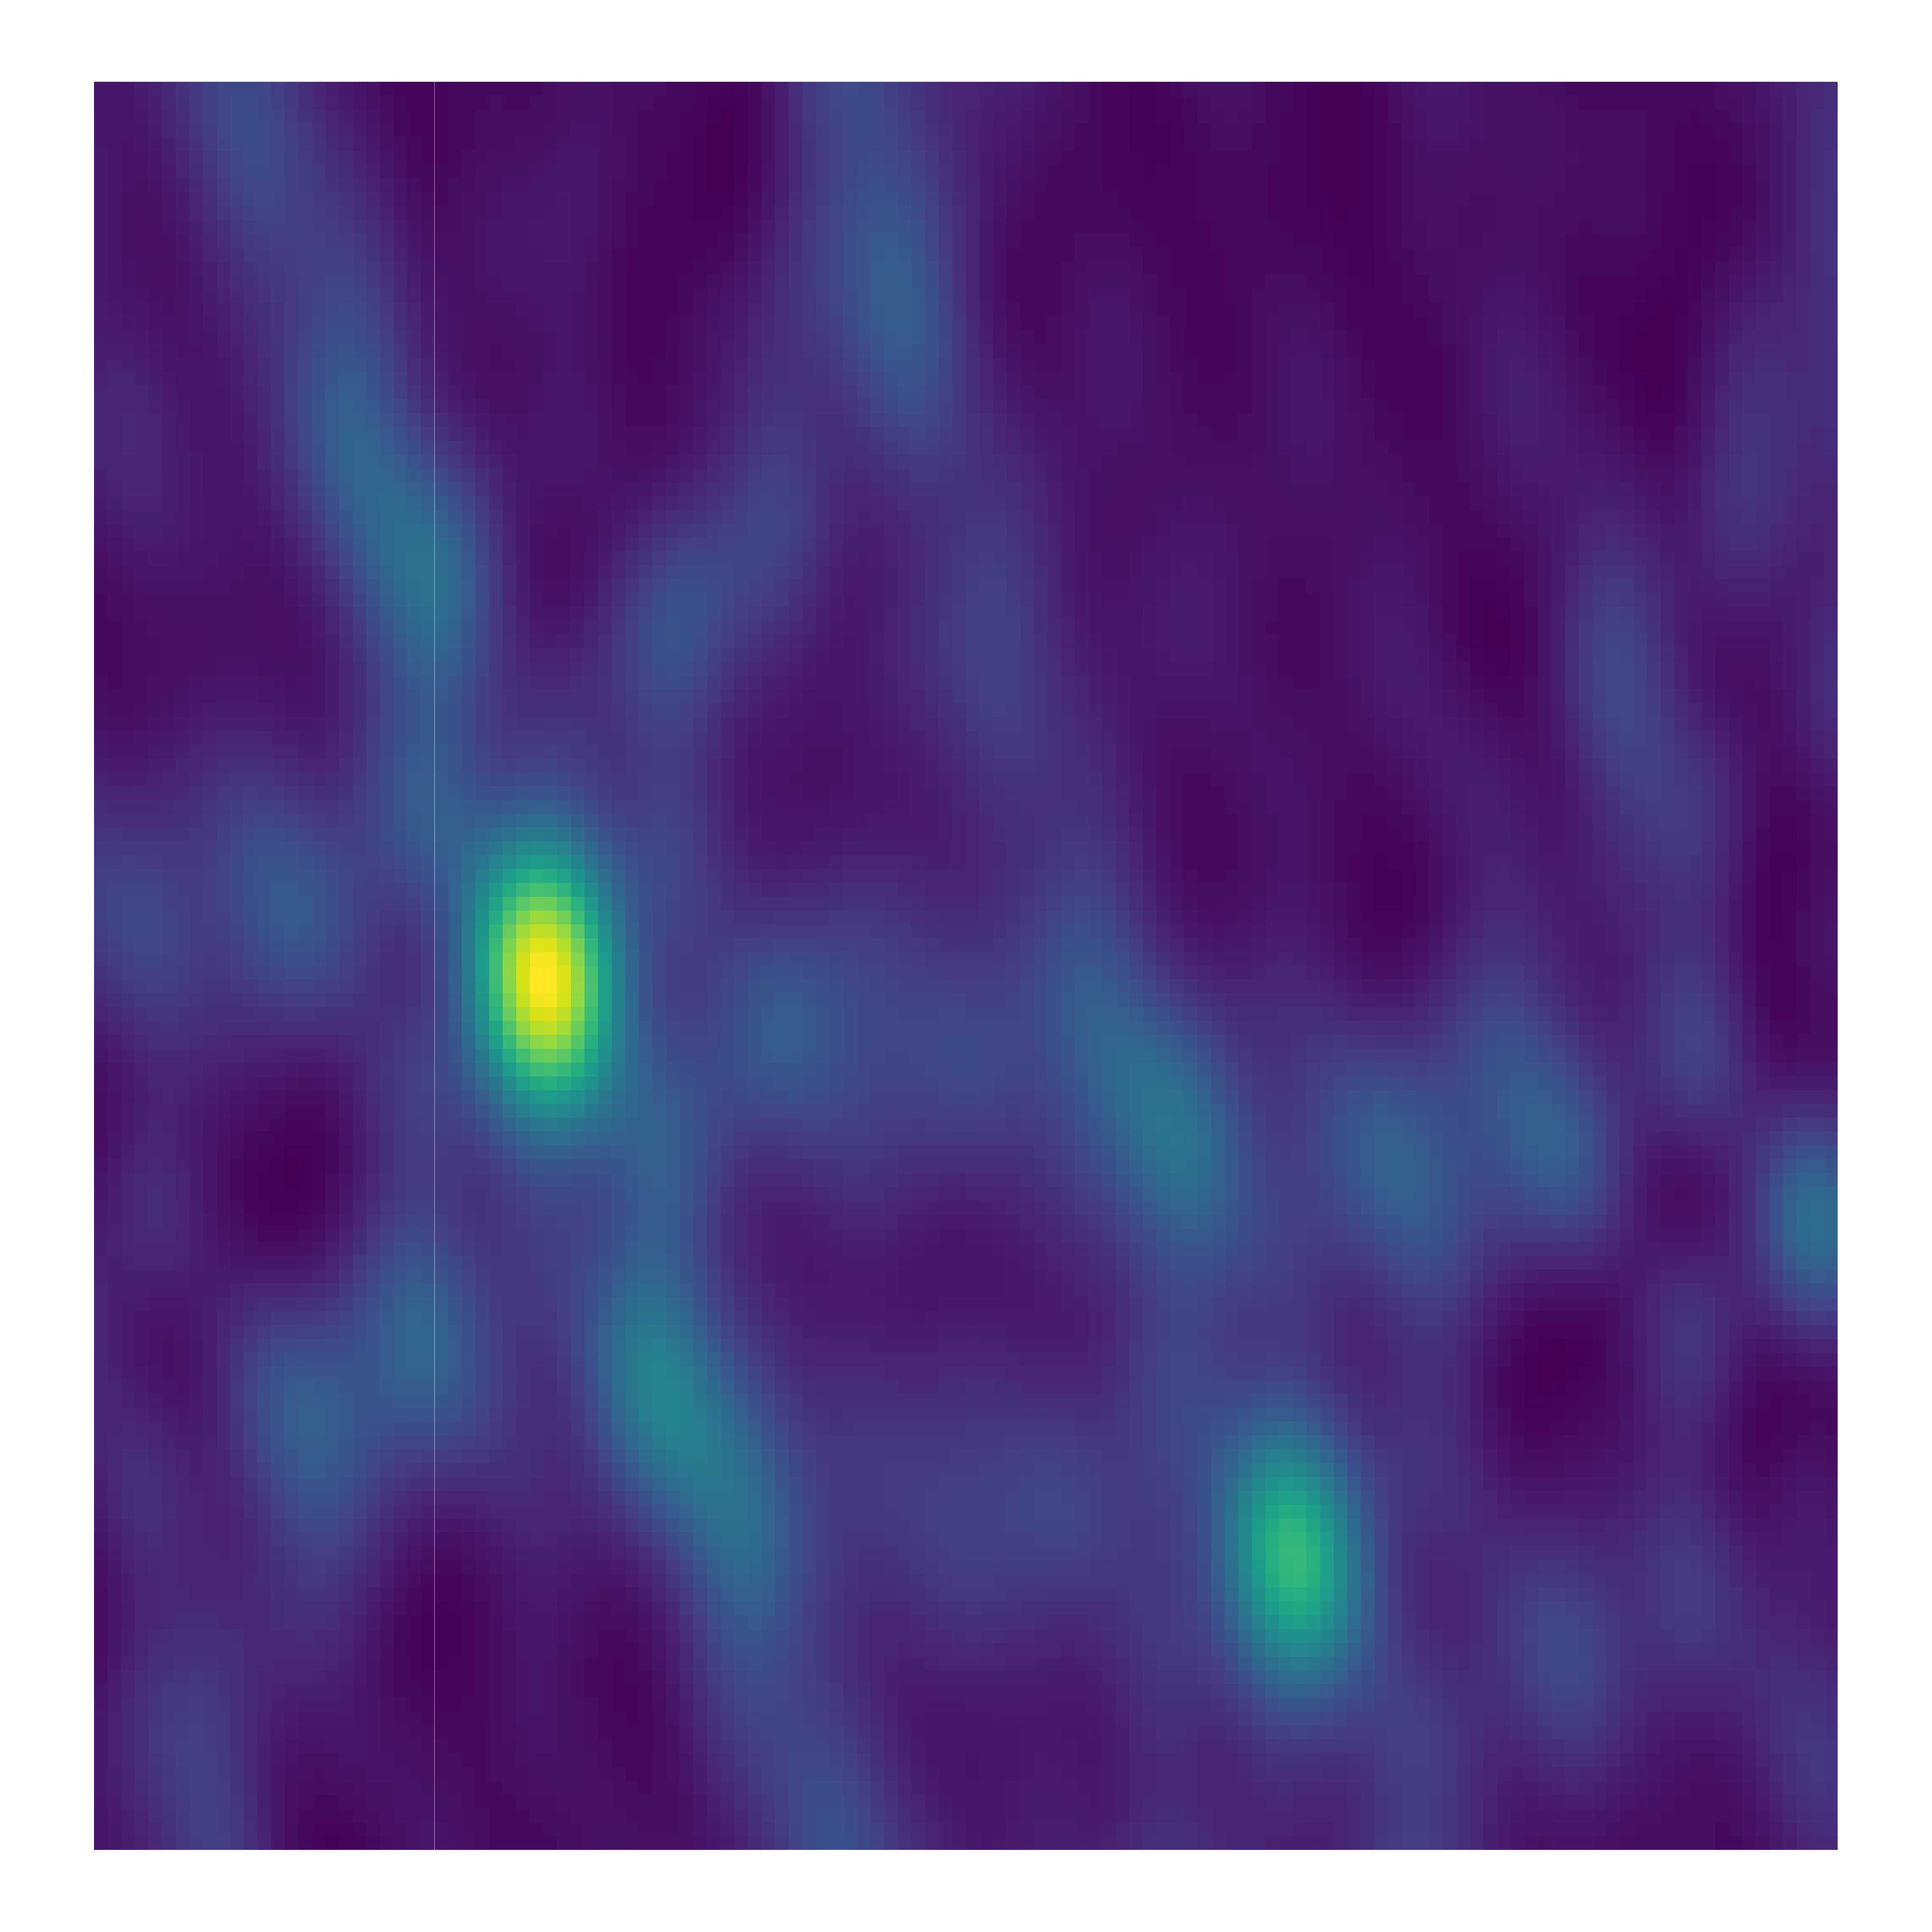
\includegraphics[width=\linewidth, trim={18px 19px 18px 18px}, clip]{./chapters/01.intro/img/dirty_image.png}
		\caption{dirty image}
	\end{subfigure}
	\begin{subfigure}[b]{0.28\linewidth}
		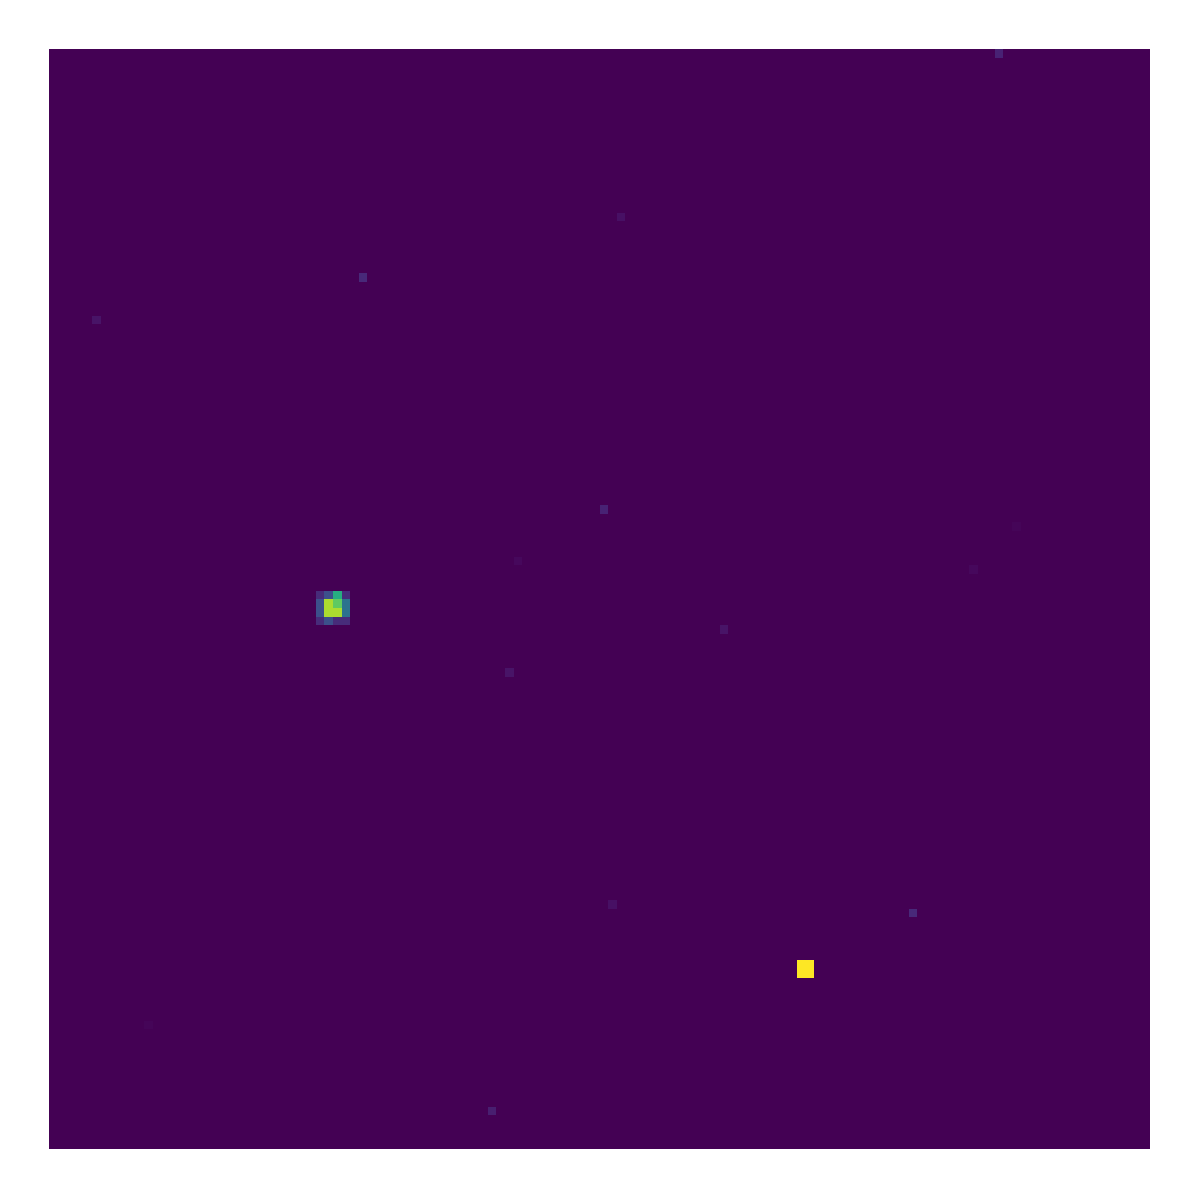
\includegraphics[width=\linewidth, trim={18px 19px 18px 18px}, clip]{./chapters/01.intro/img/true_image.png}
		\caption{true image}
	\end{subfigure}
	\caption{Deconvolution Problem VLA: Retrieve the true image when only PSF and dirty image are known}
	\label{intro:measurement_problem}
\end{figure}

%The Inverse Problem is now to remove the artefacts of the interferometer and retrieve the true image. The effects of the undersampling can be modeled by a Point Spread Function (PSF). The interferometer sees the true image of the sky, but due to undersampling it gets convolved with a PSF, resulting in the dirty image.  More formally, we try to find a solution $x$ for equation \eqref{intro:eq:deconvolve}, where only the PSF and $I_{dirty}$ are known. This problem is ill-posed: it may have multiple solutions, and a small change in the $I_{dirty}$ or the PSF may result in large changes in $x$. Furthermore, the whole problem gets corrupted by noise.

%The PSF is surprisingly easy to calculate. The Fourier Transformed PSF equals the sampling pattern in UV-Space. Remember that a convolution in image space is a multiplication in Fourier. The effects of under-sampling in image space are a convolution with the PSF. In the Fourier space it is masking all components other than the measured ones. From the Antenna Configuration we can infer the masking matrix $M$ in UV-Space. Calculating the Inverse Fourier Transform of $M$ results in the PSF.


\subsection{Approximation with CLEAN}
CLEAN assumes the observed image contains several bright point sources. In each iteration of CLEAN, it searches the highest peak of the dirty image and removes a fraction of the PSF. It stops until the next highest peak is below a threshold, or if the maximum number of iterations was reached. The fraction of the PSF, threshold and number of iterations are all tunable by the user.

It works as an approximation of the original problem. It greedily minimizes the objective \eqref{intro:eq:clean}. 
Note that the L0 norm\footnote{This is a common abuse of notation in Compressed Sensing literature: The "L0 norm" is not a norm.} acts as the indicator\footnote{For the L0 norm to work we need to define $0^0 = 0$} function.

\begin{equation}\label{intro:eq:clean}
\underset{x}{minimize} \: \left \| I_{dirty} - x \star PSF \right \|_2^2 + \: \left \| x \right \|_0
\end{equation}

Regularization term, minimum, non-convex function (It may have local minima). 
The L0 "norm" makes this problem for non-convex: It may  it is in NP-Hard. There exist optimizer like Matching Pursuit that approximate the solution well enough for practice.

but CLEAN does not minimize to an optima, it stops early. Hard to analyse how close the current solution is to the true minimum.

%beam-width

CLEAN does a greedy approximation of the deconvolution problem, and assumes the resulting image consists out of a few point sources. The question remains, how close the CLEAN approximation is to the true image? If the true image consists out of a few point sources, CLEAN produces a good approximation. Extended emissions however get approximated by a large number of faint point sources. The peak of extended emissions are generally lower than of point sources. CLEAN has more trouble distinguishing extended sources from noise. Future interferometers like MeerKAT will become more sensitive to fainter sources. The reconstruction task for new instruments may contain more faint and extended sources. Ideally, we would modify the regularization of CLEAN and explicitly model the new effects. Sadly, the regularization is a fixed part of the CLEAN algorithm.


\subsection{The Compressed Sensing Framework for Image Reconstruction}
An image reconstruction algorithm in the Compressed Sensing Framework consists of three parts:

\begin{itemize}
	\item A prior function $p()$.
	\item An optimization algorithm.
	\item An objective with a data and regularization term.
\end{itemize}

CLEAN is a Compressed Sensing Reconstruction algorithm with specific choices for prior, optimization algorithm. and objective. The prior $p()$ in CLEAN is the L0 "norm", Matching Pursuit as the optimization algorithm. The objective from CLEAN needs a additional parameter $\lambda$.  which represents the tradeoff between accurate deconvolution and regularization. the more noisy it is, the more regularization is needed. We arrive at the similar \eqref{intro:eq:csclean}.

\begin{equation}\label{intro:eq:csclean}
\underset{x}{minimize} \: \left \| D_{dirty} - x \star PSF \right \|_2^2 \: + \: \lambda \: p(x) 
\end{equation}

All that was changes was an additional parameter $\lambda$, so why would one want to do this? 
Applying non-convex optimization techniques,
Theoretical guarantees of compressed Sensing.
Replacing $p()$ with anything else

Now we can minimize \eqref{intro:eq:csclean} with non-convex optimization techniques, we can analyse how calculate lower limits for the objective.


We assume $x$ assumes the $x$ contains a few point sources. In Compressed Sensing terminology, it assumes $x$ is sparse in image space. Since $x$ is already an image.


Compressed sensing reconstruction is able to reconstruct the observation even from undersampled measurements. Even though shannon-nyquist theorem is higher.

The guarantees of Compressed Sensing Reconstruction: Incoherent from the measurement space and sparse space is sparse.

Incoherence is easy. Interferometers measure in the Fourier space(This is an approximation for small field of view imaging. The approximation breaks apart in wide field of view). The image space is maximally incoherent from the Fourier space. Intuitively, A change in a single pixel will change all fourier components. A change in a single fourier component, changes all pixels.

maximize the information gained for each element in the sparse space.

The sparse space is here to distinguish true image from unlikely candidates. It models our prior knowledge.

Then, one can reconstruct the true image from undersampled measurements. How many measurements are needed? that depends on how sparse it is. 

Taking again CLEAN as an example, if we know the image contains only one point source, we can locate it with only a few Visibilities. However if the image contains many point sources located closely together, we need more Visibilities.

The average case analysis is not trivial, 

The prior and the optimization algorithm are disconnected and the prior $p()$ can be replaced for example with the L2 norm.

%In the Compressed Sensing Framework, an approach is split into three separate parts. To demonstrate the flexibility of the Compressed Sensing Framework, we convert CLEAN into a Compressed Sensing approach.

% First we add a regularization term to \eqref{intro:eq:clean} and arrive at the new objective \eqref{intro:eq:csclean}. The objective contains the original CLEAN data term and a new regularization term. The data term forces the reconstruction to be close to the measurement, while the regularization term forces the reconstruction to be plausible. $\lambda$ models the expected noise in the problem. Note that the $\left \| Px \right \|_0$ acts as an indicator function. 

%The last step is choosing a similar optimization algorithm: In every iteration, CLEAN searches the highest peak in the dirty image. Matching Pursuit is a greedy optimization algorithm. In every iteration it searches the step which minimizes \eqref{intro:eq:csclean} the most. This Compressed Sensing approach is similar to CLEAN, but the new objective has a unique global minimum even with the presence of noise. The tunable parameters of CLEAN are replaced by a single parameter $\lambda$. 

%The strength of Compressed Sensing Framework is its flexibility: The CLEAN prior works well on point sources, but is not ideal for extended emissions. In this Framework, the prior $P$ can be replaced without changing the objective or the optimization algorithm. This has led to increased interest in Compressed Sensing for wide Field of View imaging.




